\documentclass{article}

\usepackage{amsmath}
\usepackage{nicefrac}
\usepackage{diffcoeff}
\usepackage{amsmath}
\usepackage{tcolorbox}
\usepackage{tikz}
\tikzstyle{box}=[draw, fill=red!20, minimum size=2em]

\title{AMATH 383 Project}
\author{
    Alyssa Baksh, 
    Ciaran Neely,
    Gianna Biino,
    Zaheer Mohideen
}

\begin{document}

    \maketitle

    \section{Abstract}
    \section{Introduction}
    Social networks and movements have been a crucial part of society and open a window to explaining many phenomena such as herd mentality and what causes individuals to participate in social movements \cite{diani_networks_2013}. Opinions, values or grievances is often not enough to induce actions. Connections to people participating in a social movement are generally needed to make people act \cite{small_movements_2021}.
    
    Social movements themselves are a sociological analytical concept defined as networks of interactions, may they be informal or not, between different individuals, groups and organizations, who are engaged in political or cultural conflicts, on the basis of a shared collective identity. In other words, the important aspects that need to be considered, when defining the dynamics of a social movement are: 
    \begin{itemize}
    \item It needs to be a network based on informal interactions between groups and/or organisations and individuals.
    \item It needs to contain a collective solidarity and shared beliefs.
    \item It needs to engage in conflicts, cultural or political, and promote or dispute social change.
    \item  For the majority of it, the action needs to be outside of routine and institutional procedures of social life.
    \end{itemize}
    Thanks to the broad definition of these aspects, the concept can be adapted to specific examles. If, for example, one study focuses on a global anti-systemic social movement another will focus on a social movement supporting a local system and opposing changes to it. \cite{diani_concept_1992}
    
    With the recent surge of social media, the studies of social movements and networks have evolved again, prompting further inquiries on the topic\cite{kumar_structure_2006}.
    
    Many studies have started to compare how movements founded upon social media compare to those in the past that weren't\cite{kidd_social_2016}. For example, the transnational movement in Italy was analyzed to see how digital media, like Facebook, was used by activists to spread their message, considering the number of posts, likes and comments over the  years \cite{pavan_digital_2019}. 
    
    Other studies looked at international movements. For example, one on the \textit{Black Lives Matter} movement, considering multiple social media platforms and the level of engagement of accounts. This study also discussed the limitations of social media. On one hand, traditional forms of organization still play an important role to sustain and build a movement. On the other hand, through the accessibility of social media, it is hard to maintain the actual goal and values of a movement, since many people can participate who might have different goals in mind. It is also easier for individuals to contradict the movement online by spreading opposing messages. The benefits of social media however, outweigh the costs, as it allows for a bigger scaling of social movements and a broader audience can be reached. \cite{mundt_scaling_2018}

    
    Using mathematical models, we aim to gain a deeper understanding how social movements progress with time over social media and if we can find a pattern between social movements and various parameters Specifically, we hope to find which parameters and what values are necessary for a social movement to spread and how can they be used as tools in order to spread a message.

    \section{Methods}

    
    Let $I(t)$ be the number of people engaged in the social movement at time t, and let $E(t)$ be the number of social media users who are aware of the movement at time t. Let $S(t)$ be the number of active social media users at time t who are not aware of the movement at all, and let $P(t)$ be the population of the community where the social movement is taking place. 
    
    We can relate our model equations to a type of SEIR model where $I(t)$ is the number of infected individuals, who are able to spread the disease to $S(t)$ who are the number of Susceptible people. In our case, this would mean people actively engaged in the movement would be exposing social media users through posts. 
    
    
    $E(t)$ acts as the exposed population, those who have come in contact with the disease, or in our case, those who have in come contact with the social movement by seeing social media posts about it. Similarly to how exposed individuals have a chance of becoming infected or going back to susceptible, in our model, those who are exposed to the movement can decide if they wish to actively engage in it or go back to being a part of the susceptible, $S(t)$.
    
    \textbf{Cite SIR model...} 
    
    
    
    
    However, in our model we don’t have an $R(t)$, recovered members, because we want to focus on how efficiently people are joining the movement when exposed to social media, rather than focusing on those who are “recovering” from it. Moreover, our model also included density dependence; for the first equation, as $I(t)$ increases, that means there are more infected individuals, and thus there are fewer susceptible people to expose/infect, and thus $I'(t)$ would decrease depending on the population.
    Before we start stating our equations, we need to clarify some assumptions that our model makes when taking the population and behavior of people into consideration.

    \subsection{Assumptions}
    WHAT IS R + F is limited
    
    Some of the assumptions we'll make are listed here:
    \begin{enumerate}
    \item  Everyone has equal access to social media, and our S(t) only focuses on active social media users.
    
    \item We won't consider a particular social media platform or consider different platforms as a parameter, but rather social media in general. 
    
    \item We divide the population into two parts, labelling those who use social media as S(t) and those won't don't as P(t). 
    
    \item We'll consider a closed population which means people who aren't concerned about movement, won't share posts on social media. 
    
    \item The movement does not experience significant external interventions or disruptions. For example, there isn't an opposing movement that's causing members to leave the other. 
    
    \item The movement does not have significant internal divisions or conflicts that affect its growth and spread.
    
    \item The platform used for the movement has a stable user base and does not experience significant changes in its user base or functionality.

    \item The population of the community where the movement is taking place is relatively stable and does not experience significant demographic changes.

    \item Social media overload can cause people to disengage from the movement and the platform.
    
    \item  The only way people can engage or become aware of the movement is through social media, particularly through posts that are being sent only by people already actively engaging in the movement, called infleuncers. 
    
    \item  We assume that after some time posts tend to lost traction and no longer become trending. Thus, there can only exist a certain number of trending posts at any given period of time $t$.That is, $F(t)$ is a bounded function with maximum equal to $k_8$. 

    \item Influencers all have the same rate of being able to influence others (i.e there aren’t particularly more famous/influential online celebrities that are boosting the cause). 

    \item People are equally likely to see trending posts. Once they do, they immediately become ``exposed" and then decide if they would like to join the movement or not. 
    
    \item People who leave the movement or decide not to join the movement after becoming exposed still use social media, so are then part of S(t). We assume they just forget their recent exposure/involvement with the movement and are completely unaware of it until they are exposed another time. 
    \end{enumerate}
    \subsection{Model Equations}

     Let $I(t)$ be the number of people engaged in the social movement at time $t$, and let $E(t)$ be the number of social media users who are aware of the movement at time t. Let $R(t)$ be the number of people recovering from using social media, meaning they stop using it completely. Let $S(t)$ be the number of active social media users at time t, let $P(t)$ be the population of the community where the social movement is taking place, let N(t) be the complete population of the community, and let $F(t)$ is the number of trending posts related to the movement at time $t$;\\
     \begin{figure}
         \centering
        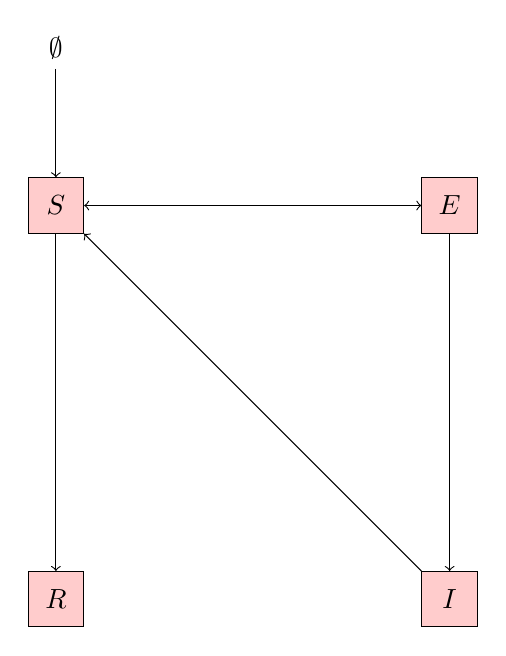
\begin{tikzpicture}
            \node [box] (S) {$S$};
            \node [box, right of=S, node distance=5cm] (E) {$E$};
            \node [box, below of=E, node distance=5cm] (I) {$I$};
            \node [box, below of=S, node distance=5cm] (R) {$R$};
            \node [above of=S, node distance=2cm] (out) {$\emptyset$};
            \path[<->] (S) edge (E);
            \path[->] (E) edge (I);
            \path[->] (I) edge (S);
            \path[->] (S) edge (R);
            \path[->] (out) edge (S);
        \end{tikzpicture}
        \caption{A diagram of the model}
    \end{figure}
    \\
    Then, the following equations can be used:
    \begin{subequations}
    \begin{align}            
        \diff St &= k_6 P(t) + k_2I(t) + k_5E(t) - k_3 {S(t)I(t)}- k_7S(t)-k_4 F(t)S(t)
        \\[10pt]
        \diff Et &= k_3 I(t)S(t) + k_4 F(t) S(t) - k_5E(t) - k_1E(t)\left[1 - \frac{I(t)}{S(t)}\right] 
        \\[10pt]
        \diff It &= k_1 E(t) \left[1 - \frac{I(t)}{S(t)}\right] - k_2I(t)
        \\[10pt]
        \diff Rt &= k_7S(t)
    \end{align}
    \end{subequations}
    
    where
    \begin{subequations}
    \begin{align}
        P(t) &= N - S(t) - E(t) - I(t)
        \\[10pt]
        F(t) &= k_8\sqrt{\frac{I(t)} N}
    \end{align}
    \end{subequations}

    and where
    \begin{itemize}
        \item $k_1^{-1}$ is the minimum expected number of weeks it takes for a person to go from $E$ to $I$;
        \item $k_2^{-1}$ is the expected number of weeks for a active member to leave the movement;
        \item $k_3$ is the rate at which social media users become exposed/aware of the movement (measured in $[\text{people}]^{-1}\times[\text{weeks}]^{-1}$);
        \item $k_4$ is the rate at which influencers promote the movement ; TODO
        \item $k_5^{-1}$ is the expected number of weeks an exposed person disengages from the movement;
        \item $k_6$ is the rate at which the non social media using population (of the community where the movement is taking place) joins social media (measured in $[\text{weeks}]^{-1}$);
        \item $k_7$ is the expected number of weeks for a person to leave the platform due to social media overload or other factors; and
        \item $k_8$ is the maximum number of trending posts that can be absorbed by a single person (measured in [posts]).
    \end{itemize}
    
    The first equation describes how the size of the movement changes over time, with the number of people becoming engaged in the movement being proportional to the number of social media users who are aware of it and the available population who may join the movement, but also subject to a rate of disengagement. 
    
	The second equation describes how the awareness of the movement changes over time, with the number of social media users becoming aware of it being proportional to the number of users who are already aware of it, as well as the rate at which influencers promote it. The rate of awareness is also subject to a rate of disengagement due to social media overload, which is proportional to the product of the number of social media users and the number of people engaged in the movement. 
 
	The third equation describes how the number of active social media users changes over time, with the number of users increasing due to population growth and social media adoption, but also subject to a rate of decline due to social media overload or other factors, which is proportional to the product of the number of social media users and the number of people engaged in the movement relative to the population size. 
 
	These equations can be used to model the growth and spread of a social movement on social media while accounting for factors such as population growth, adoption, and overload. The parameters can be adjusted to reflect the specific characteristics of the movement and the social media platforms being used.
 

    \subsection{Cases}
    
    There are certain cases we can take into consideration and analyze depending on the parameters $k_1$ through $k_8$. Some of these cases are: 


    \subsubsection*{Case 1: Rapid growth followed by quick decline, $k_1 \gg k_5$} \normalfont
    \begin{tcolorbox}
    Assuming that $k_1$  is much greater than $k_5$, the social movement is likely to experience rapid growth as more and more social media users become engaged and stay involved. However, if $k_2$ (rate of actively engaged people leaving the movement) is also high, the movement could fizzle out quickly as actively engaged individuals leave. If it was low, the movement could continue to grow and attract even more engaged individuals.
    \subsubsection*{Conclusion}  The movement could experience rapid growth in its initial stages, but depending on $k_2$, it could quickly decline. Therefore, it is important to strike a balance between retaining engaged individuals and allowing individuals who no longer align with the movement's goals to leave, in order to ensure the long-term success and impact of the movement.
    \end{tcolorbox}

    \subsubsection*{Case 2: Struggling to gain traction, $k_3 < k_1$ and $k_3 < k_5$}
    \begin{tcolorbox}
    Assuming that $k_3$ is much smaller than $k_1$ and $k_5$, the social movement may struggle to gain traction as social media users are not becoming aware of the movement at a fast enough rate, and exposed individuals are disengaging quickly. However, if the rate at which influencers promote the movement ($k_4$) is high, then the movement could still gain traction and attract more engaged individuals, despite a slow initial growth.
    \subsubsection*{Conclusion} The movement  struggles to gain momentum and grow but may gain some traction if $k_4$ is high. Therefore, it is important to consider both the rate of exposure to the movement and the influence of key individuals in promoting and sustaining momentum for the movement.
    \end{tcolorbox}
    
    \subsubsection*{Case 3: Influencers driving movement forward, $k_4 > k_5$} \normalfont
    \begin{tcolorbox}
     In this case, influencers could play a key role in driving the movement forward by promoting it frequently. The movement is more likely to gain momentum and have a lasting impact. This is because influencers can help sustain engagement and encourage continued participation even as individuals may be exposed to negative or disengaging factors. By promoting the movement and highlighting its benefits and impact, influencers can motivate individuals to become engaged and invested in the movement. This can help sustain participation over time and mitigate the potential negative effects of disengagement  exposed individuals.
    \subsubsection*{Conclusion}Tthe movement could continue to grow and thrive, even if some exposed individuals disengage. This case underscores the importance of the role of influencers in promoting a social movement and sustaining engagement over time. 
    \end{tcolorbox}



    \subsubsection*{Case 4: Sudden spike in engagement but high risk of burnout, $k_6 > k_3$ \normalfont{and} $k_6 > k_5$}
    \begin{tcolorbox}
   In this case, the movement has the potential to rapidly gain momentum and reach a wide audience. As more individuals in the community join social media, they become exposed to the movement and may become engaged and invested in its goals and objectives. This can help sustain momentum and encourage continued participation, particularly if efforts are made to retain engaged individuals and address negative factors contributing to disengagement. 
   
   However, it is also important to consider the potential challenges associated with rapid growth and expansion. As the movement gains momentum and reaches a wider audience, it may become more difficult to maintain cohesion and direction, particularly if there are diverse opinions and perspectives  participants.
    \subsubsection*{Conclusion} In summary,  the case highlights the potential benefits and challenges associated with rapid growth and expansion in a social movement. By complementing efforts to increase visibility and engagement with broader strategies to manage growth and maintain cohesion, social movements can maximize their impact and reach a wider audience.
    \end{tcolorbox}

    \subsubsection*{Case 5: $k_3 > k_6$}
    \begin{tcolorbox}
    In this case, the movement may struggle to gain traction and expand its reach beyond initial participants.
    
    While efforts to raise awareness of the movement among existing social media users may help to generate initial interest and support, the movement may struggle to expand its reach beyond this initial group without effective strategies for engaging individuals who are not already using social media.
    
    In such a scenario, it may be useful to consider strategies for increasing social media adoption among non-users, such as targeted advertising or outreach efforts. Additionally, efforts to establish partnerships with organizations and groups outside of social media can help to generate broader support and reach individuals who may not be engaged through social media alone.
    \subsubsection*{Conclusion}
    The movement is likely to plateau and fails to reach new individuals. The case highlights the potential challenges associated with relying solely on social media to promote and sustain a social movement. By complementing efforts to increase awareness and engagement on social media with strategies for engaging non-users and establishing partnerships with organizations outside of social media, social movements can maximize their impact and expand their reach beyond initial participants.
    \end{tcolorbox}

    \subsubsection*{Case 6: $k_4 > k_5$ \normalfont{and} $k_8 > k_7$}
    \begin{tcolorbox}
    In this case, influencers are effectively promoting the movement ($k_4 > k_5$) and social media users are leaving the platform at a slower rate than they are joining it ($k_8 > k_7$). This means that while social media may be overwhelming some users, it's still an effective tool for spreading awareness and engaging new supporters.
    \subsubsection*{Conclusion}
    The movement is likely to continue growing in popularity, but social media may need to find ways to reduce user overload and keep existing users engaged.
    \end{tcolorbox}

    \section{Results}
    \section{Discussion}
    \newpage
    \bibliographystyle{plain}
    \bibliography{references}
    

\end{document}